% Caminhos mínimos em grafos

Algoritmo de Dijkstra
======================

- Descoberto em {\bf 1959} por Edsger Wybe Dijkstra (1930--2002).

 \includegraphics[scale=0.3]{img/dijkstrapaperheader.png}  

Ideia
======

\tikzstyle{vertex}=[circle,fill=black!25,minimum size=20pt,inner sep=0pt]
\tikzstyle{edge} = [draw,thick,->,>=latex]
\tikzstyle{weight} = [font=\small]
\tikzstyle{selected edge} = [draw,line width=3pt,->,>=latex,red!70]

\begin{columns}
  \begin{column}{0.325\textwidth}

\only<1>{
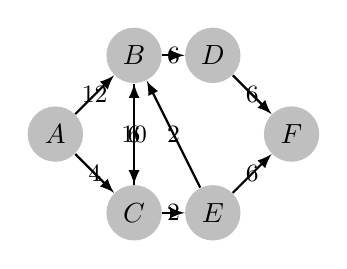
\begin{tikzpicture}
\foreach \pos/\name in {{(0,0)/A}, {(1,1)/B}, {(1,-1)/C},
                         {(2,1)/D}, {(2,-1)/E}, {(3,0)/F}}{
  \node[vertex] (\name) at \pos {$\name$};
}
\foreach \source/\dest/\weight/\isselected in {A/B/12/0, A/C/4/0, B/C/6/0,
                                   B/D/6/0, C/B/10/0, C/E/2/0,
                                   D/F/6/0, E/B/2/0, E/F/6/0} {
  \ifnum\isselected=0                                   
  \path[edge] (\source) -- node[weight] {$\weight$} (\dest);
  \else
  \path[selected edge] (\source) -- node[weight] {$\weight$} (\dest);
  \fi
}
\end{tikzpicture}
}


\only<2>{
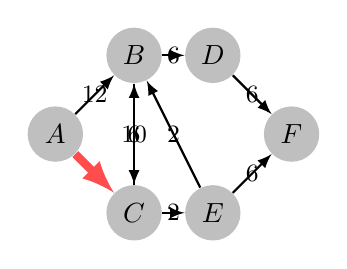
\begin{tikzpicture}
\foreach \pos/\name in {{(0,0)/A}, {(1,1)/B}, {(1,-1)/C},
                         {(2,1)/D}, {(2,-1)/E}, {(3,0)/F}}{
  \node[vertex] (\name) at \pos {$\name$};
}
\foreach \source/\dest/\weight/\isselected in {A/B/12/0, A/C/4/1, B/C/6/0,
                                   B/D/6/0, C/B/10/0, C/E/2/0,
                                   D/F/6/0, E/B/2/0, E/F/6/0} {
  \ifnum\isselected=0                                   
  \path[edge] (\source) -- node[weight] {$\weight$} (\dest);
  \else
  \path[selected edge] (\source) -- node[weight] {$\weight$} (\dest);
  \fi
}
\end{tikzpicture}
}
 \only<3>{
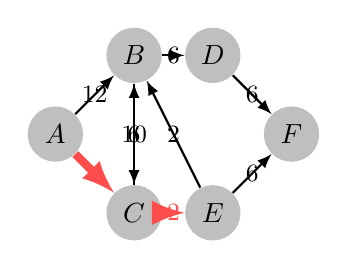
\begin{tikzpicture}
\foreach \pos/\name in {{(0,0)/A}, {(1,1)/B}, {(1,-1)/C},
                         {(2,1)/D}, {(2,-1)/E}, {(3,0)/F}}{
  \node[vertex] (\name) at \pos {$\name$};
}
\foreach \source/\dest/\weight/\isselected in {A/B/12/0, A/C/4/1, B/C/6/0,
                                   B/D/6/0, C/B/10/0, C/E/2/1,
                                   D/F/6/0, E/B/2/0, E/F/6/0} {
  \ifnum\isselected=0                                   
  \path[edge] (\source) -- node[weight] {$\weight$} (\dest);
  \else
  \path[selected edge] (\source) -- node[weight] {$\weight$} (\dest);
  \fi
}
\end{tikzpicture}
}

 \only<4>{
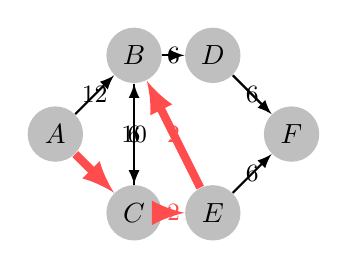
\begin{tikzpicture}
\foreach \pos/\name in {{(0,0)/A}, {(1,1)/B}, {(1,-1)/C},
                         {(2,1)/D}, {(2,-1)/E}, {(3,0)/F}}{
  \node[vertex] (\name) at \pos {$\name$};
}
\foreach \source/\dest/\weight/\isselected in {A/B/12/0, A/C/4/1, B/C/6/0,
                                   B/D/6/0, C/B/10/0, C/E/2/1,
                                   D/F/6/0, E/B/2/1, E/F/6/0} {
  \ifnum\isselected=0                                   
  \path[edge] (\source) -- node[weight] {$\weight$} (\dest);
  \else
  \path[selected edge] (\source) -- node[weight] {$\weight$} (\dest);
  \fi
}
\end{tikzpicture}
}

 \only<5>{
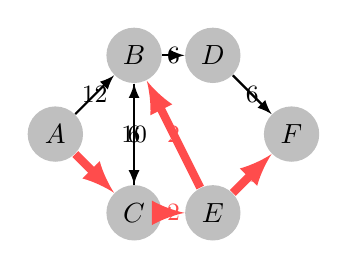
\begin{tikzpicture}
\foreach \pos/\name in {{(0,0)/A}, {(1,1)/B}, {(1,-1)/C},
                         {(2,1)/D}, {(2,-1)/E}, {(3,0)/F}}{
  \node[vertex] (\name) at \pos {$\name$};
}
\foreach \source/\dest/\weight/\isselected in {A/B/12/0, A/C/4/1, B/C/6/0,
                                   B/D/6/0, C/B/10/0, C/E/2/1,
                                   D/F/6/0, E/B/2/1, E/F/6/1} {
  \ifnum\isselected=0                                   
  \path[edge] (\source) -- node[weight] {$\weight$} (\dest);
  \else
  \path[selected edge] (\source) -- node[weight] {$\weight$} (\dest);
  \fi
}
\end{tikzpicture}
}

 \only<6>{
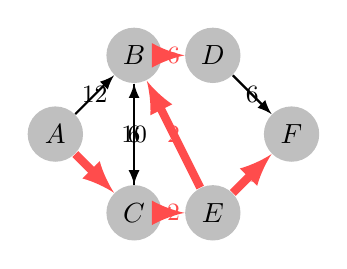
\begin{tikzpicture}
\foreach \pos/\name in {{(0,0)/A}, {(1,1)/B}, {(1,-1)/C},
                         {(2,1)/D}, {(2,-1)/E}, {(3,0)/F}}{
  \node[vertex] (\name) at \pos {$\name$};
}
\foreach \source/\dest/\weight/\isselected in {A/B/12/0, A/C/4/1, B/C/6/0,
                                   B/D/6/1, C/B/10/0, C/E/2/1,
                                   D/F/6/0, E/B/2/1, E/F/6/1} {
  \ifnum\isselected=0                                   
  \path[edge] (\source) -- node[weight] {$\weight$} (\dest);
  \else
  \path[selected edge] (\source) -- node[weight] {$\weight$} (\dest);
  \fi
}
\end{tikzpicture}
  
}

\end{column}

\begin{column}{0.6\textwidth}
\scriptsize
\only<1>{
\begin{tabular}{|c|c|c|c|c|c|c|}\hline
  & A & B & C & D & E & F \\\hline\hline
Distância & 0&1000 & 1000& 1000&1000 & 1000\\\hline
Anterior & -- &-- &-- &-- &-- &-- \\\hline
\end{tabular}
}

\only<2>{
\begin{tabular}{|c|c|c|c|c|c|c|}\hline
          & A$^*$ & B   & C$^*$& D  & E   & F   \\\hline\hline
Distância & 0 &1000 & {\bf 4}& 1000&1000 & 1000\\\hline
Anterior & -- & A & A & -- & -- &-- \\\hline
\end{tabular}
}

\only<3>{
\begin{tabular}{|c|c|c|c|c|c|c|}\hline
          & A$^*$ & B   & C$^*$& D  & E$^*$   & F   \\\hline\hline
Distância & 0   & 12  & {\bf 4}& 1000& {\bf 6} & 1000\\\hline
Anterior & -- & A & A &-- & C &-- \\\hline
\end{tabular}
}

\only<4>{
\begin{tabular}{|c|c|c|c|c|c|c|}\hline
          & A$^*$ & B$^*$   & C$^*$& D  & E$^*$   & F   \\\hline\hline
Distância & 0   & {\bf 8}  & {\bf 4}& 1000& {\bf 6} & 10\\\hline
Anterior & -- & E & A &-- & C &E \\\hline
\end{tabular}
}
\only<5>{
\begin{tabular}{|c|c|c|c|c|c|c|}\hline
          & A$^*$ & B$^*$   & C$^*$& D  & E$^*$   & F$^*$   \\\hline\hline
Distância & 0   & {\bf 8}  & {\bf 4}& 14& {\bf 6} & {\bf 10}\\\hline
Anterior & -- & E & A & B & C &E \\\hline
\end{tabular}
}

 \only<6>{   
\begin{tabular}{|c|c|c|c|c|c|c|}\hline
          & A$^*$ & B$^*$   & C$^*$& D$^*$  & E$^*$   & F$^*$   \\\hline\hline
Distância & 0   & {\bf 8}  & {\bf 4}& {\bf 14}& {\bf 6} & {\bf 10}\\\hline
Anterior & -- & E & A & B & C &E \\\hline
\end{tabular}
}

\end{column}
\end{columns}

\vspace{0.75cm}

\begin{center}
\begin{scriptsize}
    \begin{tabular}{|c|c|c|c|c|c|c|}\hline
        & A    & B   & C   & D   & E   & F \\\hline\hline
      A & 0    &12   & 4   & 1000&1000 & 1000\\\hline
      B & 1000 &0    & 6   & 6   &1000 & 1000\\\hline
      C & 1000 &10   & 0   & 1000&2    & 1000\\\hline
      D & 1000 &1000 & 8   & 0   &1000 & 6\\\hline
      E & 1000 &2    & 1000& 1000&0    & 6\\\hline
      F & 1000 &1000 & 1000& 1000&1000 & 0\\\hline
    \end{tabular}
  \end{scriptsize}
\end{center}
